%-----------------------------------------------------------------------------------------
% Autor dieser Vorlage:
% Stefan Macke (http://fachinformatiker-anwendungsentwicklung.net)
% Permalink zur Vorlage: http://fiae.link/LaTeXVorlageFIAE
%
% Sämtliche verwendeten Abbildungen, Tabellen und Listings stammen von Dirk Grashorn.
%
% Lizenz: Creative Commons 4.0 Namensnennung - Weitergabe unter gleichen Bedingungen
% -----------------------------------------------------------------------------------------

\documentclass[
	ngerman,
	toc=listof, % Abbildungsverzeichnis sowie Tabellenverzeichnis in das Inhaltsverzeichnis aufnehmen
	toc=bibliography, % Literaturverzeichnis in das Inhaltsverzeichnis aufnehmen
	footnotes=multiple, % Trennen von direkt aufeinander folgenden Fußnoten
	parskip=half, % vertikalen Abstand zwischen Absätzen verwenden anstatt horizontale Einrückung von Folgeabsätzen
	numbers=noendperiod % Den letzten Punkt nach einer Nummerierung entfernen (nach DIN 5008)
]{scrartcl}
\usepackage[utf8]{inputenc} % muss als erstes eingebunden werden, da Meta/Packages ggfs. Sonderzeichen enthalten

\usepackage{luatex85}
\pdfminorversion=5 % erlaubt das Einfügen von pdf-Dateien bis Version 1.7, ohne eine Fehlermeldung zu werfen (keine Garantie für fehlerfreies Einbetten!)

% !TEX root = Projektdokumentation.tex

\providecommand{\pruefungstermin}{Winter 2025/2026} % <anpassen>
\providecommand{\ausbildungsberuf}{Fachinformatiker / Anwendungsentwicklung}
\providecommand{\betreff}{Projektdokumentation} % <anpassen>
\providecommand{\betriebLogo}{Bilder/ananas_codes.png} 

\providecommand{\titel}{Empfehlungsmarketing-App}
\providecommand{\untertitel}{Webanwendung zur Empfehlungslinkerstellung und Gutscheingenerierung}
\providecommand{\autorName}{Benjamin Blunk}
\providecommand{\autorAnschrift}{Auf dem Schild 6}
\providecommand{\autorOrt}{23560 Lübeck}
\providecommand{\betriebName}{ananas.codes e.K.}
\providecommand{\betriebAnschrift}{Lindenstraße 8}
\providecommand{\betriebOrt}{23558 Lübeck}
\providecommand{\abgabeOrt}{Lübeck}
\providecommand{\abgabeTermin}{10.12.2025}
 % Metadaten zu diesem Dokument (Autor usw.)
% !TEX root = ../Projektdokumentation.tex

% Anpassung an Landessprache ---------------------------------------------------
\usepackage{babel}
\usepackage[utf8]{inputenc}
% \usepackage[ngerman]{babel}


%   Erlaubt automatische Trennung von Worten mit Umlauten.
% ------------------------------------------------------------------------------
\usepackage[T1]{fontenc}
\usepackage{textcomp} % Euro-Zeichen etc.

% Schrift ----------------------------------------------------------------------
\usepackage{lmodern} % bessere Fonts
\usepackage{relsize} % Schriftgröße relativ festlegen

% Tabellen ---------------------------------------------------------------------
\PassOptionsToPackage{table}{xcolor}
\usepackage{tabularx}
% für lange Tabellen
\usepackage{longtable}
\usepackage{array}
\usepackage{ragged2e}
\usepackage{lscape}
\newcolumntype{w}[1]{>{\raggedleft\hspace{0pt}}p{#1}} % Spaltendefinition rechtsbündig mit definierter Breite
% Neuer Spaltentyp: linksbündig + vertikal zentriert
\newcolumntype{L}[1]{>{\raggedright\arraybackslash}m{#1}}
% Grafiken ---------------------------------------------------------------------
\usepackage[dvips,final]{graphicx} % Einbinden von JPG-Grafiken ermöglichen
% \usepackage{graphics} % keepaspectratio
\usepackage{floatflt} % zum Umfließen von Bildern
\graphicspath{{Bilder/}} % hier liegen die Bilder des Dokuments

% Sonstiges --------------------------------------------------------------------
\usepackage[titles]{tocloft} % Inhaltsverzeichnis DIN 5008 gerecht einrücken
\usepackage{amsmath,amsfonts} % Befehle aus AMSTeX für mathematische Symbole
\usepackage{enumitem} % anpassbare Enumerates/Itemizes
\usepackage{xspace} % sorgt dafür, dass Leerzeichen hinter parameterlosen Makros nicht als Makroendezeichen interpretiert werden
\usepackage{xcolor}
\usepackage{tikz}
\usepackage[T1]{fontenc}
\usetikzlibrary{matrix, shapes, positioning, arrows.meta, fit, backgrounds}
\usepackage{caption}

\usepackage{makeidx} % für Index-Ausgabe mit \printindex
\usepackage[printonlyused]{acronym} % es werden nur benutzte Definitionen aufgelistet

% Einfache Definition der Zeilenabstände und Seitenränder etc.
\usepackage{setspace}
\usepackage{geometry}

% Symbolverzeichnis
\usepackage[intoc]{nomencl}
\let\abbrev\nomenclature
\renewcommand{\nomname}{Abkürzungsverzeichnis}
\setlength{\nomlabelwidth}{.25\hsize}
\renewcommand{\nomlabel}[1]{#1 \dotfill}
\setlength{\nomitemsep}{-\parsep}

\usepackage{varioref} % Elegantere Verweise. „auf der nächsten Seite“
\usepackage{url} % URL verlinken, lange URLs umbrechen etc.

\usepackage{chngcntr} % fortlaufendes Durchnummerieren der Fußnoten
% \usepackage[perpage]{footmisc} % Alternative: Nummerierung der Fußnoten auf jeder Seite neu

\usepackage{ifthen} % bei der Definition eigener Befehle benötigt
\usepackage{todonotes} % definiert u.a. die Befehle \todo und \listoftodos
\usepackage[square]{natbib} % wichtig für korrekte Zitierweise

% PDF-Optionen -----------------------------------------------------------------
\usepackage{pdfpages}
\pdfminorversion=5 % erlaubt das Einfügen von pdf-Dateien bis Version 1.7, ohne eine Fehlermeldung zu werfen (keine Garantie für fehlerfreies Einbetten!)
\usepackage[
    bookmarks,
    bookmarksnumbered,
    bookmarksopen=true,
    bookmarksopenlevel=1,
    colorlinks=true,
% diese Farbdefinitionen zeichnen Links im PDF farblich aus
    anchorcolor=AOBlau,% Ankertext
    citecolor=AOBlau, % Verweise auf Literaturverzeichniseinträge im Text
    filecolor=AOBlau, % Verknüpfungen, die lokale Dateien öffnen
    menucolor=AOBlau, % Acrobat-Menüpunkte
    urlcolor=AOBlau,
% diese Farbdefinitionen sollten für den Druck verwendet werden (alles schwarz)
    %linkcolor=black, % einfache interne Verknüpfungen
    %anchorcolor=black, % Ankertext
    %citecolor=black, % Verweise auf Literaturverzeichniseinträge im Text
    %filecolor=black, % Verknüpfungen, die lokale Dateien öffnen
    %menucolor=black, % Acrobat-Menüpunkte
    %urlcolor=black,
%
    %backref, % Quellen werden zurück auf ihre Zitate verlinkt
    pdftex,
    plainpages=false, % zur korrekten Erstellung der Bookmarks
    pdfpagelabels=true, % zur korrekten Erstellung der Bookmarks
    hypertexnames=false, % zur korrekten Erstellung der Bookmarks
    linkcolor=black,
    linktoc=all,
]{hyperref}
% Befehle, die Umlaute ausgeben, führen zu Fehlern, wenn sie hyperref als Optionen übergeben werden
\hypersetup{
    pdftitle={\titel -- \untertitel},
    pdfauthor={\autorName},
    pdfcreator={\autorName},
    pdfsubject={\titel -- \untertitel},
    pdfkeywords={\titel -- \untertitel},
}


% zum Einbinden von Programmcode -----------------------------------------------
\usepackage{listings}
\usepackage{xcolor}
\definecolor{hellgelb}{rgb}{1,1,0.9}
\definecolor{colKeys}{rgb}{0,0,1}
\definecolor{colIdentifier}{rgb}{0,0,0}
\definecolor{colComments}{rgb}{0,0.5,0}
\definecolor{colString}{rgb}{1,0,0}
\lstset{
    float=hbp,
	basicstyle=\footnotesize,
    identifierstyle=\color{colIdentifier},
    keywordstyle=\color{colKeys},
    stringstyle=\color{colString},
    commentstyle=\color{colComments},
    backgroundcolor=\color{hellgelb},
    columns=flexible,
    tabsize=2,
    frame=single,
    extendedchars=true,
    showspaces=false,
    showstringspaces=false,
    numbers=left,
    numberstyle=\tiny,
    breaklines=true,
    breakautoindent=true,
	captionpos=b,
}
\lstdefinelanguage{cs}{
	sensitive=false,
	morecomment=[l]{//},
	morecomment=[s]{/*}{*/},
	morestring=[b]",
	morekeywords={
		abstract,event,new,struct,as,explicit,null,switch
		base,extern,object,this,bool,false,operator,throw,
		break,finally,out,true,byte,fixed,override,try,
		case,float,params,typeof,catch,for,private,uint,
		char,foreach,protected,ulong,checked,goto,public,unchecked,
		class,if,readonly,unsafe,const,implicit,ref,ushort,
		continue,in,return,using,decimal,int,sbyte,virtual,
		default,interface,sealed,volatile,delegate,internal,short,void,
		do,is,sizeof,while,double,lock,stackalloc,
		else,long,static,enum,namespace,string},
}
\lstdefinelanguage{natural}{
	sensitive=false,
	morecomment=[l]{/*},
	morestring=[b]",
	morestring=[b]',
	alsodigit={-,*},
	morekeywords={
		DEFINE,DATA,LOCAL,END-DEFINE,WRITE,CALLNAT,PARAMETER,USING,
		IF,NOT,END-IF,ON,*ERROR-NR,ERROR,END-ERROR,ESCAPE,ROUTINE,
		PERFORM,SUBROUTINE,END-SUBROUTINE,CONST,END-FOR,END,FOR,RESIZE,
		ARRAY,TO,BY,VALUE,RESET,COMPRESS,INTO,EQ},
}
\lstdefinelanguage{php}{
	sensitive=false,
	morecomment=[l]{/*},
	morestring=[b]",
	morestring=[b]',
	alsodigit={-,*},
	morekeywords={
		abstract,and,array,as,break,case,catch,cfunction,class,clone,const,
		continue,declare,default,do,else,elseif,enddeclare,endfor,endforeach,
		endif,endswitch,endwhile,extends,final,for,foreach,function,global,
		goto,if,implements,interface,instanceof,namespace,new,old_function,or,
		private,protected,public,static,switch,throw,try,use,var,while,xor
		die,echo,empty,exit,eval,include,include_once,isset,list,require,
		require_once,return,print,unset},
}

% Umlaute ----------------------------------------------------------------------
%   Umlaute/Sonderzeichen wie äüöß direkt im Quelltext verwenden (CodePage).
\lstset{
  literate=
    {ä}{{\"a}}1
    {ö}{{\"o}}1
    {ü}{{\"u}}1
    {Ä}{{\"A}}1
    {Ö}{{\"O}}1
    {Ü}{{\"U}}1
    {ß}{{\ss}}1
} % verwendete Packages
% !TEX root = ../Projektdokumentation.tex

% Seitenränder -----------------------------------------------------------------
\setlength{\topskip}{\ht\strutbox} % behebt Warnung von geometry
\geometry{
  a4paper,
  left=25mm,        % linker Rand
  right=25mm,       % rechter Rand
  top=7mm,          % oberer Rand inkl. Kopfzeile -> Kopf rückt höher
  bottom=25mm,      % unterer Rand
  includehead,      % Kopfbereich in die Berechnung einbeziehen
  includefoot,      % Fußbereich in die Berechnung einbeziehen
  headsep=8mm,      % Abstand Kopfzeile -> Textblock
  footskip=12mm     % Abstand Textblock -> Fußzeile
}

\makeatletter
\makeatother


% Kopf-/Fußzeilen mit KOMA-Script ---------------------------------------------
\usepackage[
  automark,   % Kapitel-/Abschnittsangaben in Kopfzeile automatisch erstellen
  headsepline,% Trennlinie unter der Kopfzeile
  ilines      % Trennlinie linksbündig ausrichten
]{scrlayer-scrpage}

% --- EINSTELLUNG: Höhe des Logos im Header (einfach hier ändern) -------------
\newlength{\HeaderLogoHeight}
\setlength{\HeaderLogoHeight}{23mm} % <- Höhe des Logos in der Kopfzeile

% Kopf- und Fußzeilen ----------------------------------------------------------
\clearpairofpagestyles
\pagestyle{scrheadings}

% Kopfzeile
\renewcommand{\headfont}{\normalfont} % Schriftform der Kopfzeile
\ihead{%
  \large\textsc{\titel}\\
  \small\untertitel \\[2ex]
  \textit{\headmark}%
}
\chead{}
\ohead{\includegraphics[height=\HeaderLogoHeight]{\betriebLogo}}

% Headheight passend zum Logo und Text (ohne geometry anzufassen)
\setlength{\headheight}{\dimexpr \HeaderLogoHeight + 12pt\relax}

% Fußzeile
\ifoot*{\autorName}
\cfoot*{\pagemark}   % <-- Seitenzahl jetzt zentriert
\ofoot*{}            % rechts leer

% Überschriften nach DIN 5008 in einer Fluchtlinie -----------------------------

% Abstand zwischen Nummerierung und Überschrift definieren
\newcommand{\headingSpace}{1.5cm}

% Abschnittsüberschriften im selben Stil wie beim Inhaltsverzeichnis einrücken
\renewcommand*{\othersectionlevelsformat}[3]{%
  \makebox[\headingSpace][l]{#3\autodot}%
}

% Für die Einrückung wird das Paket tocloft benötigt
\cftsetindents{section}{0.0cm}{\headingSpace}
\cftsetindents{subsection}{0.0cm}{\headingSpace}
\cftsetindents{subsubsection}{0.0cm}{\headingSpace}
\cftsetindents{figure}{0.0cm}{\headingSpace}
\cftsetindents{table}{0.0cm}{\headingSpace}

% Allgemeines ------------------------------------------------------------------
\onehalfspacing % Zeilenabstand 1,5 Zeilen
\frenchspacing  % erzeugt ein wenig mehr Platz hinter einem Punkt

% Schusterjungen und Hurenkinder vermeiden
\clubpenalty = 10000
\widowpenalty = 10000
\displaywidowpenalty = 10000

% Quellcode-Ausgabe formatieren
\lstset{numbers=left, numberstyle=\tiny, numbersep=5pt, breaklines=true}
\lstset{emph={square}, emphstyle=\color{red}, emph={[2]root,base}, emphstyle={[2]\color{blue}}}

\counterwithout{footnote}{section} % Fußnoten fortlaufend durchnummerieren
\setcounter{tocdepth}{3}           % bis subsubsection ins Inhaltsverzeichnis
\setcounter{secnumdepth}{3}        % bis subsubsection nummerieren

% Aufzählungen anpassen
\renewcommand{\labelenumi}{\arabic{enumi}.}
\renewcommand{\labelenumii}{\arabic{enumi}.\arabic{enumii}.}
\renewcommand{\labelenumiii}{\arabic{enumi}.\arabic{enumii}.\arabic{enumiii}}

% Tabellenfärbung:
\definecolor{heading}{rgb}{0.64,0.78,0.86}
\definecolor{odd}{rgb}{0.9,0.9,0.9}

% Seitenstil für Verzeichnisse: Kopf behalten, Fuß leer
\newpairofpagestyles{verzeichnis}{
  \ihead{%
    \large\textsc{\titel}\\
    \small\untertitel \\[2ex]
    \textit{\headmark}%
  }
  \chead{}
  \ohead{\includegraphics[height=\HeaderLogoHeight]{\betriebLogo}}
  % Fußzeile komplett leer:
  \ifoot{}
  \cfoot{}
  \ofoot{}
}
 % Definitionen zum Aussehen der Seiten
% !TEX root = ../Projektdokumentation.tex

% Abkürzungen, ggfs. mit korrektem Leerraum
\newcommand{\bs}{$\backslash$\xspace}
\newcommand{\bspw}{bspw.\xspace}
\newcommand{\bzw}{bzw.\xspace}
\newcommand{\ca}{ca.\xspace}
\newcommand{\dahe}{\mbox{d.\,h.}\xspace}
\newcommand{\etc}{etc.\xspace}
\newcommand{\eur}[1]{\mbox{#1\,\texteuro}\xspace}
\newcommand{\evtl}{evtl.\xspace}
\newcommand{\ggfs}{ggfs.\xspace}
\newcommand{\Ggfs}{Ggfs.\xspace}
\newcommand{\gqq}[1]{\glqq{}#1\grqq{}}
\newcommand{\inkl}{inkl.\xspace}
\newcommand{\insb}{insb.\xspace}
\newcommand{\ua}{\mbox{u.\,a.}\xspace}
\newcommand{\usw}{usw.\xspace}
\newcommand{\Vgl}{Vgl.\xspace}
\newcommand{\zB}{\mbox{z.\,B.}\xspace}

% Befehle für häufig anfallende Aufgaben
\newcommand{\Abbildung}[1]{\autoref{fig:#1}}
\newcommand{\Anhang}[1]{\appendixname{}~\ref{#1}: \nameref{#1} \vpageref{#1}}
\newcommand{\quelle}[1]{\textsuperscript{[#1]}}
\newcommand{\includegraphicsKeepAspectRatio}[2]{\includegraphics[width=#2\textwidth,height=#2\textheight,keepaspectratio]{#1}}
\newcommand{\Zitat}[2][\empty]{\ifthenelse{\equal{#1}{\empty}}{\citep{#2}}{\citep[#1]{#2}}}
\newcommand{\Autor}[1]{\textsc{#1}} % zum Ausgeben von Autoren
\newcommand{\itemd}[2]{\item{\textbf{#1}}\\{#2}} % erzeugt ein Listenelement mit fetter Überschrift

% fügt Tabellen aus einer TEX-Datei ein
\newcommand{\tabelle}[3] % Parameter: caption, label, file
{\begin{table}[htbp]
\centering
\singlespacing
\input{Tabellen/#3}
\caption{#1}
\label{#2}
\end{table}}

\newcommand{\tabelleAnhang}[1] % Parameter: file
{\begin{center}
\singlespacing
\input{Tabellen/#1}
\end{center}}

% einfaches Wechseln der Schrift, z.B.: \changefont{cmss}{sbc}{n}
\newcommand{\changefont}[3]{\fontfamily{#1} \fontseries{#2} \fontshape{#3} \selectfont}

% Verwendung analog zu \includegraphics
\newlength{\myx} % Variable zum Speichern der Bildbreite
\newlength{\myy} % Variable zum Speichern der Bildhöhe
\newcommand\includegraphicstotab[2][\relax]{%
% Abspeichern der Bildabmessungen
\settowidth{\myx}{\includegraphics[{#1}]{#2}}%
\settoheight{\myy}{\includegraphics[{#1}]{#2}}%
% das eigentliche Einfügen
\parbox[c][1.1\myy][c]{\myx}{%
\includegraphics[{#1}]{#2}}%
}

\definecolor{AOBlau}{rgb}{0, 0.28, 0.56}

% verschiedene Befehle um Wörter semantisch auszuzeichnen ----------------------
\newcommand{\Index}[2][\empty]{\ifthenelse{\equal{#1}{\empty}}{\index{#2}#2}{\index{#1}#2}}
\newcommand{\Fachbegriff}[2][\empty]{\ifthenelse{\equal{#1}{\empty}}{\textit{\Index{#2}}}{\textit{\Index[#1]{#2}}}}
\newcommand{\NeuerBegriff}[2][\empty]{\ifthenelse{\equal{#1}{\empty}}{\textbf{\Index{#2}}}{\textbf{\Index[#1]{#2}}}}

\newcommand{\Ausgabe}[1]{\texttt{#1}}
\newcommand{\Eingabe}[1]{\texttt{#1}}
\newcommand{\Code}[1]{\texttt{#1}}
\newcommand{\Datei}[1]{\texttt{#1}}

\newcommand{\Assembly}[1]{\textsf{#1}}
\newcommand{\Klasse}[1]{\textsf{#1}}
\newcommand{\Methode}[1]{\textsf{#1}}
\newcommand{\Attribut}[1]{\textsf{#1}}

\newcommand{\Datentyp}[1]{\textsf{#1}}
\newcommand{\XMLElement}[1]{\textsf{#1}}
\newcommand{\Webservice}[1]{\textsf{#1}}

\newcommand{\Refactoring}[1]{\Fachbegriff{#1}}
\newcommand{\CodeSmell}[1]{\Fachbegriff{#1}}
\newcommand{\Metrik}[1]{\Fachbegriff{#1}}
\newcommand{\DesignPattern}[1]{\Fachbegriff{#1}}
 % eigene allgemeine Befehle, die z.B. die Arbeit mit LaTeX erleichtern
% !TEX root = ../Projektdokumentation.tex

% Abkürzungen, ggfs. mit korrektem Leerraum
\newcommand{\bs}{$\backslash$\xspace}
\newcommand{\bspw}{bspw.\xspace}
\newcommand{\bzw}{bzw.\xspace}
\newcommand{\ca}{ca.\xspace}
\newcommand{\dahe}{\mbox{d.\,h.}\xspace}
\newcommand{\etc}{etc.\xspace}
\newcommand{\eur}[1]{\mbox{#1\,\texteuro}\xspace}
\newcommand{\evtl}{evtl.\xspace}
\newcommand{\ggfs}{ggfs.\xspace}
\newcommand{\Ggfs}{Ggfs.\xspace}
\newcommand{\gqq}[1]{\glqq{}#1\grqq{}}
\newcommand{\inkl}{inkl.\xspace}
\newcommand{\insb}{insb.\xspace}
\newcommand{\ua}{\mbox{u.\,a.}\xspace}
\newcommand{\usw}{usw.\xspace}
\newcommand{\Vgl}{Vgl.\xspace}
\newcommand{\zB}{\mbox{z.\,B.}\xspace}

% Befehle für häufig anfallende Aufgaben
\newcommand{\Abbildung}[1]{\autoref{fig:#1}}
\newcommand{\Anhang}[1]{\appendixname{}~\ref{#1}: \nameref{#1} \vpageref{#1}}
\newcommand{\quelle}[1]{\textsuperscript{[#1]}}
\newcommand{\includegraphicsKeepAspectRatio}[2]{\includegraphics[width=#2\textwidth,height=#2\textheight,keepaspectratio]{#1}}
\newcommand{\Zitat}[2][\empty]{\ifthenelse{\equal{#1}{\empty}}{\citep{#2}}{\citep[#1]{#2}}}
\newcommand{\Autor}[1]{\textsc{#1}} % zum Ausgeben von Autoren
\newcommand{\itemd}[2]{\item{\textbf{#1}}\\{#2}} % erzeugt ein Listenelement mit fetter Überschrift

% fügt Tabellen aus einer TEX-Datei ein
\newcommand{\tabelle}[3] % Parameter: caption, label, file
{\begin{table}[htbp]
\centering
\singlespacing
\input{Tabellen/#3}
\caption{#1}
\label{#2}
\end{table}}

\newcommand{\tabelleAnhang}[1] % Parameter: file
{\begin{center}
\singlespacing
\input{Tabellen/#1}
\end{center}}

% einfaches Wechseln der Schrift, z.B.: \changefont{cmss}{sbc}{n}
\newcommand{\changefont}[3]{\fontfamily{#1} \fontseries{#2} \fontshape{#3} \selectfont}

% Verwendung analog zu \includegraphics
\newlength{\myx} % Variable zum Speichern der Bildbreite
\newlength{\myy} % Variable zum Speichern der Bildhöhe
\newcommand\includegraphicstotab[2][\relax]{%
% Abspeichern der Bildabmessungen
\settowidth{\myx}{\includegraphics[{#1}]{#2}}%
\settoheight{\myy}{\includegraphics[{#1}]{#2}}%
% das eigentliche Einfügen
\parbox[c][1.1\myy][c]{\myx}{%
\includegraphics[{#1}]{#2}}%
}

\definecolor{AOBlau}{rgb}{0, 0.28, 0.56}

% verschiedene Befehle um Wörter semantisch auszuzeichnen ----------------------
\newcommand{\Index}[2][\empty]{\ifthenelse{\equal{#1}{\empty}}{\index{#2}#2}{\index{#1}#2}}
\newcommand{\Fachbegriff}[2][\empty]{\ifthenelse{\equal{#1}{\empty}}{\textit{\Index{#2}}}{\textit{\Index[#1]{#2}}}}
\newcommand{\NeuerBegriff}[2][\empty]{\ifthenelse{\equal{#1}{\empty}}{\textbf{\Index{#2}}}{\textbf{\Index[#1]{#2}}}}

\newcommand{\Ausgabe}[1]{\texttt{#1}}
\newcommand{\Eingabe}[1]{\texttt{#1}}
\newcommand{\Code}[1]{\texttt{#1}}
\newcommand{\Datei}[1]{\texttt{#1}}

\newcommand{\Assembly}[1]{\textsf{#1}}
\newcommand{\Klasse}[1]{\textsf{#1}}
\newcommand{\Methode}[1]{\textsf{#1}}
\newcommand{\Attribut}[1]{\textsf{#1}}

\newcommand{\Datentyp}[1]{\textsf{#1}}
\newcommand{\XMLElement}[1]{\textsf{#1}}
\newcommand{\Webservice}[1]{\textsf{#1}}

\newcommand{\Refactoring}[1]{\Fachbegriff{#1}}
\newcommand{\CodeSmell}[1]{\Fachbegriff{#1}}
\newcommand{\Metrik}[1]{\Fachbegriff{#1}}
\newcommand{\DesignPattern}[1]{\Fachbegriff{#1}}
 % eigene projektspezifische Befehle, z.B. Abkürzungen usw.

\usepackage{float}

% Hilfs-Makros für Attribute
\newcommand{\pk}[1]{\texttt{\textcolor{red!60!black}{#1}}}
\newcommand{\fk}[1]{\texttt{\textcolor{blue!60!black}{#1}}}
\newcommand{\attr}[1]{\texttt{#1}}

% \usepackage{showframe} % Debugging Element-Frames

\begin{document}

\phantomsection
% IHK-Deckblatt (als PDF), ohne Kopf/Fuß:
\pdfbookmark[1]{Eidesstattliche Erklärung}{ihkdeckblatt}
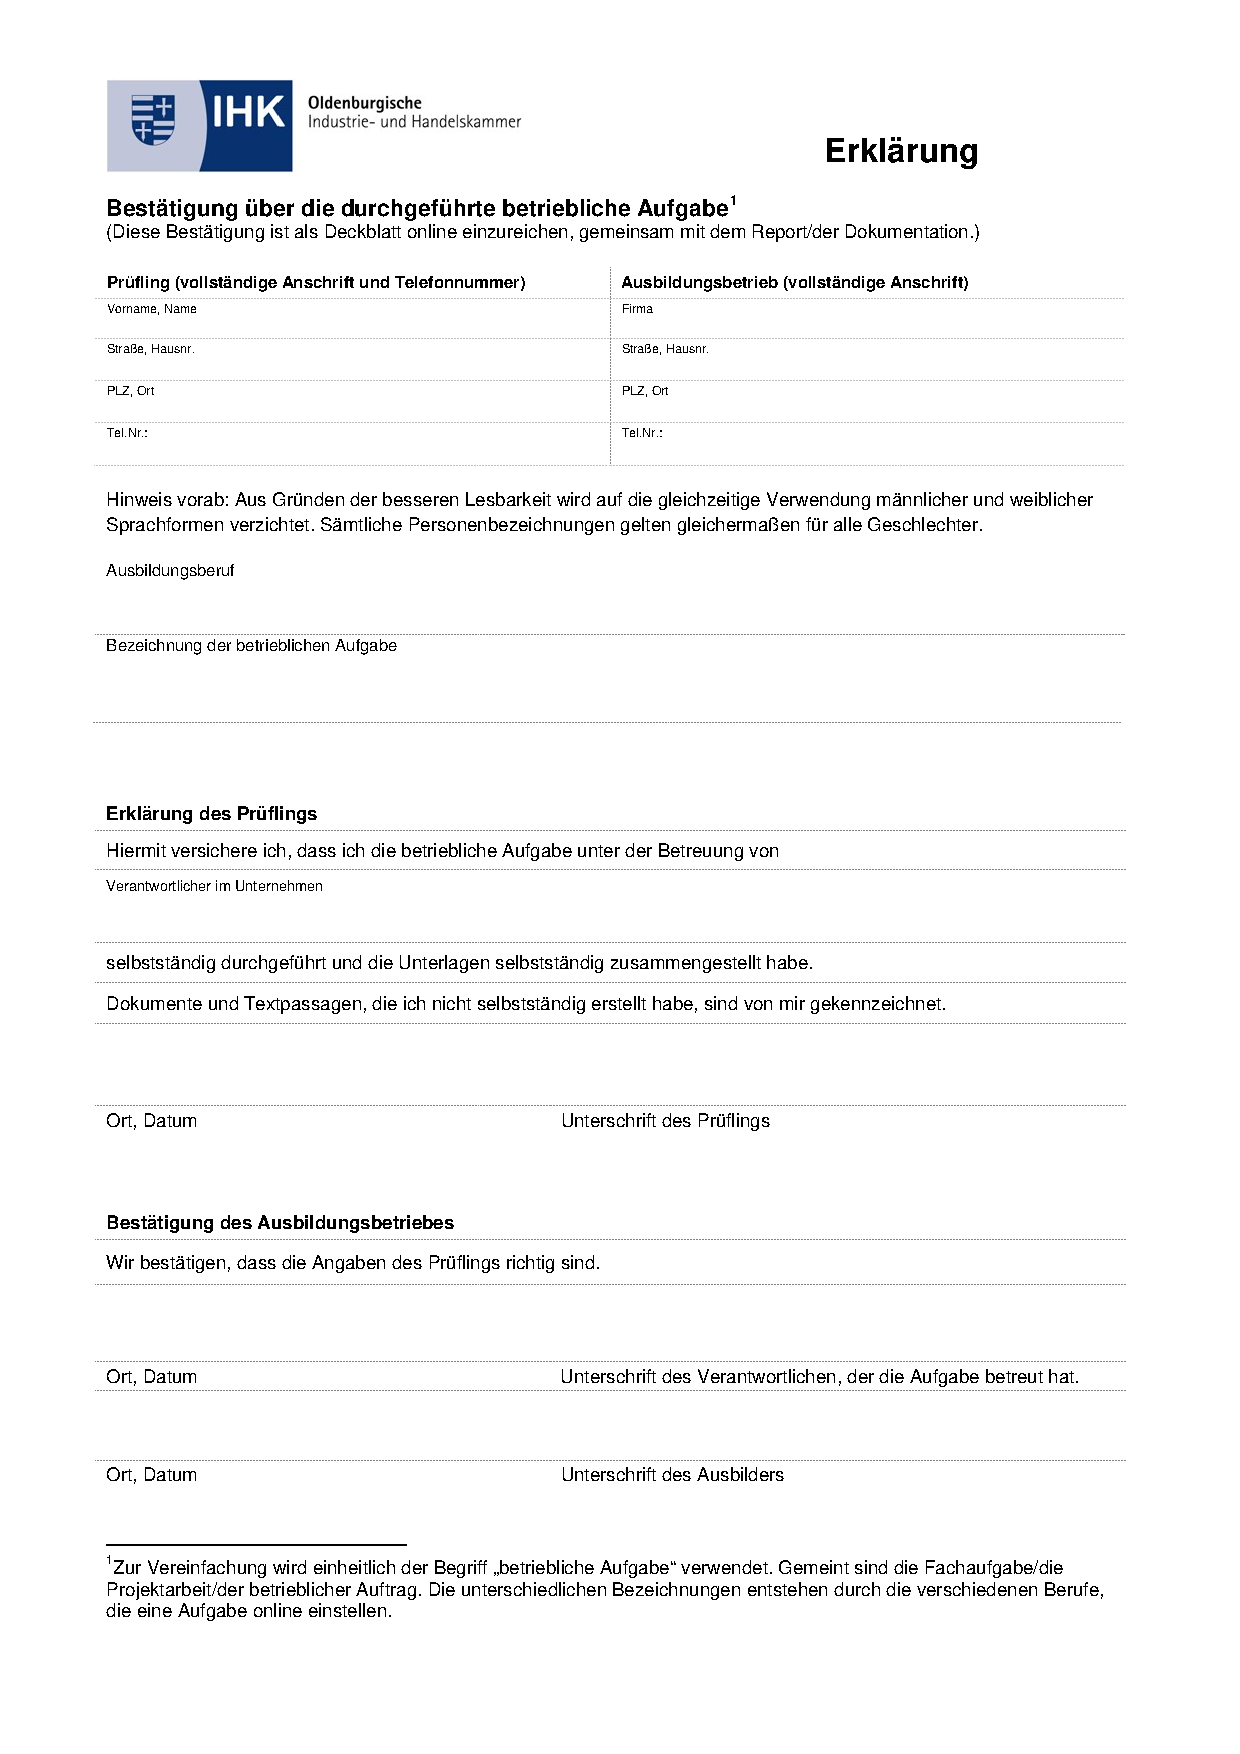
\includepdf[pages=1,pagecommand={\thispagestyle{empty}}]{Bilder/DeckblattIHK}
\clearpage

\phantomsection
\pdfbookmark[1]{Deckblatt}{deckblatt}
% !TEX root = Projektdokumentation.tex

% Temporär: Kopf-/Fußbereiche NICHT berücksichtigen, damit echte Seitenmitte gilt
\newgeometry{
  left=25mm, right=25mm, top=25mm, bottom=25mm,
  includehead=false, includefoot=false
}

\begin{titlepage}
  \pagestyle{empty}    % gesamte Seite ohne Kopf-/Fußzeile
  \thispagestyle{empty}

  \begin{center}
    \vspace*{\fill}
    \begin{minipage}{0.9\textwidth}
      \centering

      
\includegraphics[height=18mm]{LogoIHK.pdf}\\[1ex]
      \Large{Abschlussprüfung \pruefungstermin}\\[3ex]

      \Large{\ausbildungsberuf}\\
      \LARGE{\betreff}\\[4ex]

      \huge{\textbf{\titel}}\\[1.5ex]
      \Large{\textbf{\untertitel}}\\[4ex]

      \normalsize
      Abgabetermin: \abgabeOrt, den \abgabeTermin\\[3em]
      \textbf{Prüfungsbewerber:}\\
      \autorName\\
      \autorAnschrift\\
      \autorOrt\\[5ex]

      \textbf{Ausbildungsbetrieb:}\\
      \betriebName\\
      \betriebAnschrift\\
      \betriebOrt\\[5em]

      
\includegraphics[height=35mm]{Bilder/ananas_codes.png}\\[2ex]
    \end{minipage}
    \vspace*{\fill}
  \end{center}

  % Titelblatt-Seite wirklich leer lassen (KOMA setzt am Ende gerne 'plain'):
  \thispagestyle{empty}
\end{titlepage}

\restoregeometry

\clearpage

% Inhaltsverzeichnis ----------------------------------------------------------
\phantomsection
\pagenumbering{Roman}
\pdfbookmark[1]{Inhaltsverzeichnis}{inhalt}

\pagestyle{verzeichnis}
\tableofcontents
\clearpage

% Abkürzungsverzeichnis -------------------------------------------------------
\newcommand{\abkvz}{Abkürzungsverzeichnis}
\renewcommand{\nomname}{\abkvz}
\section*{\abkvz}
\markboth{\abkvz}{\abkvz}
\addcontentsline{toc}{section}{\abkvz}

\pagestyle{verzeichnis}
% !TEX root = Projektdokumentation.tex

% Es werden nur die Abkürzungen aufgelistet, die mit \ac definiert und auch benutzt wurden. 
%
% \acro{VERSIS}{Versicherungsinformationssystem\acroextra{ (Bestandsführungssystem)}}
% Ergibt in der Liste: VERSIS Versicherungsinformationssystem (Bestandsführungssystem)
% Im Text aber: \ac{VERSIS} -> Versicherungsinformationssystem (VERSIS)

% Hinweis: allgemein bekannte Abkürzungen wie z.B. bzw. u.a. müssen nicht ins Abkürzungsverzeichnis aufgenommen werden
% Hinweis: allgemein bekannte IT-Begriffe wie Datenbank oder Programmiersprache müssen nicht erläutert werden,
%          aber ggfs. Fachbegriffe aus der Domäne des Prüflings (z.B. Versicherung)

% Die Option (in den eckigen Klammern) enthält das längste Label oder
% einen Platzhalter der die Breite der linken Spalte bestimmt.
\begin{acronym}[WWWWW]
	\acro{AES}{Advanced Encryption Standard}\acused{API}
	\acro{API}{Application Programming Interface}\acused{API}
	\acro{CDN}{Content-Delivery-Network}\acused{CDN}
	\acro{Cloud}{Web-Server}\acused{Cloud}
	\acro{CSRF}{Cross-Site Request Forgery}\acused{CSRF}
	\acro{CSS}{Cascading Style Sheets}\acused{CSS}
	\acro{DOM}{Document Object Model}\acused{DOM}
	\acro{DSGVO}{Datenschutzgrundverordnung}\acused{DSGVO}
	\acro{EPK}{Ereignisgesteuerte Prozesskette}\acused{EPK}
	\acro{ERM}{En\-ti\-ty-Re\-la\-tion\-ship-Mo\-dell}
        \acro{FTP}{File Transfer Protocol}\acused{FTP}
        \acro{Git}{verteiltes Versionsverwaltungssystem}\acused{Git}
        \acro{GitHub}{Plattform für Git-Repositories}\acused{GitHub}
        \acro{GUI}{Graphical User Interface}\acused{GUI}
	\acro{HTML}{Hypertext Markup Language}\acused{HTML}
	\acro{PDF}{Portable Document Format}\acused{PDF}
	\acro{PDO}{PHP Data Object}\acused{PDO}
	\acro{PHP}{Hypertext Preprocessor}\acused{PHP}
	\acro{QR}{Quick Response}\acused{QR}
	\acro{SSL/TLS}{Secure Sockets Layer/Transport Layer Security}\acused{SSL/TLS}
	\acro{SQL}{Structured Query Language}\acused{SQL}
	\acro{UI}{User Interface}\acused{UI}
	\acro{UML}{Unified Modeling Language}\acused{UML}
	\acro{URL}{Uniform Resource Locator}\acused{URL}
	\acro{VS Code}{Visual Studio Code - Code-Editor von Microsoft}\acused{VS Code}
	\acro{XML}{Extensible Markup Language}\acused{XML}
	\acro{ZXing}{Ausgesprochen: „Zebra Crossing“. Open-Source-Bibliothek zur Erkennung und in einigen Implementierungen auch zur Erstellung von Barcodes und QR-Codes.}\acused{ZXing}
	\acro{@zxing/browser}{Ausgesprochen: Zebra Crossing. Bibliothek zum Scannen von Bar-           und QR-Codes}\acused{@zxing/browser}
\end{acronym}

\clearpage

% Inhalt ---------------------------------------------------------------------
\clearpage
\pagenumbering{arabic}
\pagestyle{scrheadings}
% !TEX root = Projektdokumentation.tex
% Inhalt.tex – Aggregator für Kapiteldateien
% !TEX root = ../Projektdokumentation.tex
\section{Einleitung}
\label{sec:Einleitung}

\subsection{Begriffsklärung}
\label{sec:Begriffsklaerung}
Zur Gewährleistung einer konsistenten und verständlichen Verwendung von Begriffen innerhalb dieser Projektdokumentation werden folgende Festlegungen getroffen:
\begin{itemize}
    \item Der \textbf{Kunde}, der seinen Empfehlungslink an Interessenten weiter gibt, wird im weiteren Verlauf als \textbf{Werber} bezeichnet.
    \item Der \textbf{Interessent} wird im weiteren Verlauf als der \textbf{Geworbene} bezeichnet.
\end{itemize}
Durch diese Vereinheitlichung soll die Lesbarkeit und Nachvollziehbarkeit der Dokumentation verbessert werden.

\subsection{Projektumfeld} 
\label{sec:Projektumfeld}
\begin{itemize}
	\item Mein Praktikumsbetrieb ist die Firma ananas.codes e.K., welche im Bereich Webentwicklung und Zeiterfassungssysteme tätig ist. Die Mitarbeiteranzahl beträgt aktuell acht.
	\item Der Auftraggeber ist die Colibri Contactlinsen und Brillen GmbH, welche aktuell eine Filiale und eine Zweigstelle in Lübeck hat und insgesamt vierzig Mitarbeiter beschäftigt.
\end{itemize}


\subsection{Projektziel} 
\label{sec:Projektziel}
\begin{itemize}
	\item Es geht um die Entwicklung einer Empfehlungsmarketing-Webanwendung.
	\item Das Ziel des Projekts war die Konzeption, Entwicklung und Einführung einer webbasierten Empfehlungsmarketing-Applikation für einen realen Kundenbetrieb.
    Die Anwendung soll es ermöglichen:
    \begin{itemize}
    \item Kunden über einen Registrierungsprozess in ein Empfehlungsprogramm aufzunehmen.
    \item Empfehlungslinks inklusive QR-Codes zu generieren und per E-Mail zu versenden.
    \item Gutscheine automatisch auszustellen und Einlösungen im Mitarbeiterbereich vorzunehmen.
    \item Den gesamten Prozess sicher, \acs{DSGVO} konform und plattformunabhängig abzuwickeln.    
    \end{itemize}
Die Entwicklung erfolgte als eigenständiges Projekt im Rahmen der Abschlussprüfung, orientiert an den Phasen des Wasserfallmodells.
\end{itemize}

\subsection{Projektbegründung} 
\label{sec:Projektbegruendung}
\begin{itemize}
	\item Gewinnung von Neukunden durch Affiliates\quelle{1}.
	\item Der Auftraggeber möchte über solch eine moderne Form der Neukundengewinnung verfügen.
	\item Die Branchen-Software des Auftraggebers unterstützt kein Empfehlungsmarketing.
\end{itemize}


\subsection{Projektschnittstellen} 
\label{sec:Projektschnittstellen}
Die Anwendung besteht aus einem webbasierten Frontend (\ac{HTML}, \ac{CSS}, JavaScript, Bootstrap\quelle{3}) und einem serverseitigen Backend (\ac{PHP}, Composer\quelle{2}, MySQL\quelle{7}).  
Die Kommunikation zwischen Frontend und Backend erfolgt über die \texttt{Fetch-API\quelle{4}} mittels \ac{HTTPS}-Requests.  
Daten werden dabei im \ac{JSON}-Format ausgetauscht.  

\begin{itemize}
    \item \textbf{Frontend $\longrightarrow$ Backend:}
    \begin{itemize}
        \item[$\rightarrow$] Über \texttt{fetch()}-Aufrufe werden REST-ähnliche Endpunkte in \texttt{api.php} angesprochen.
        \item[$\rightarrow$] Scanner-Funktion: Im Mitarbeiterbereich wird ein QR-Code-Scanner (\texttt{@zxing/browser} Bibliothek) genutzt, um Gutscheincodes zu erfassen.
    \end{itemize}

    \item \textbf{Backend $\longrightarrow$ Datenbank / interne Systeme:}
    \begin{itemize}
        \item[$\rightarrow$] Speicherung und Validierung von Benutzer- und Gutscheindaten in einer Datenbank.
        \item[$\rightarrow$] Prüfung und Generierung eindeutiger Referral-Codes ohne Kollision.
        \item[$\rightarrow$] Hashing und Fingerprinting von E-Mail-Adressen für Datenschutz.
        \item[$\rightarrow$] Versand von E-Mails (inklusive QR-Code-Anhang) über ein internes Mailer-System.
    \end{itemize}

    \item \textbf{Genehmigung:}
    \begin{itemize}
        \item[$\rightarrow$] Das Projekt wird vom Chef meines Praktikumsbetriebs genehmigt.
    \end{itemize}

    \item \textbf{Benutzer der Anwendung:}
    \begin{itemize}
        \item[$\rightarrow$] Werber, die sich registrieren und ihren Empfehlungslink teilen, um Gutscheine zu erhalten.
        \item[$\rightarrow$] Geworbene, die sich registrieren um ihren Empfehlungslink und einen Gutschein zu erhalten.
        \item[$\rightarrow$] Mitarbeiter, die Gutscheincodes scannen und einlösen, wenn diese erfolgreich validiert wurden.
    \end{itemize}

    \item \textbf{Präsentation der Ergebnisse:}
    \begin{itemize}
        \item[$\rightarrow$] Die Projektergebnisse werden meinem Chef präsentiert.
    \end{itemize}
\end{itemize}

\subsection{Projektabgrenzung} 
\label{sec:Projektabgrenzung}
\begin{itemize}
	\item Meine Projektarbeit umfasst die Entwicklung des Frontend und Backend der Anwendung, sowie das Testen und die abschließende Abnahme durch meinen Chef. Der Rollout beim Kunden ist nicht Bestandteil meiner Projektarbeit.
\end{itemize}

\section{Projektplanung}
\label{sec:Projektplanung}

\subsection{Projektphasen}
\label{sec:Projektphasen}
Es wurde das Wasserfallmodell eingesetzt:
\begin{itemize}
  \item \textbf{Analyse}
  \item \textbf{Entwurf}
  \item \textbf{Implementierung}
  \item \textbf{Test}
  \item \textbf{Wartung}
\end{itemize}

\subsection{Abweichungen vom Projektantrag}
\label{sec:AbweichungenProjektantrag}

\begin{itemize}
  \item Detaillierte Projektbeschreibung
        \begin{itemize}
          \item Die Angabe, dass der Geworbene nur einen Rabatt erhält wenn er eine Brille kauft ist nicht richtig. Es wird vom Auftraggeber noch entschieden, für welche Produkte eine Rabattierung möglich ist.
          \item Dem Geworbenen wird ebenfalls ein Affiliate-Link zusätzlich zum Gutschein zugesandt, da dieser dann ebenfalls einen Anreiz hat diesen zu teilen um weitere Gutscheine zu erhalten.
          \item Die Angabe, dass die Gutscheine ihre Gültigkeit nicht verlieren sollen beruht auf einem Missverständnis zwischen mir und meinem Chef. Die Gutscheine sollen nach der Einlösung entwertet werden.
          \item Die Frontend-Library qr-scanner wird ersetzt durch \ac{ZXing} für den QR-Code-Scan zum Einlösen von Gutscheinen, da diese Library häufig genutzt wird in der Softwareentwicklung und sehr zuverlässig und schnell QR-Codes erkennt.
        \end{itemize}
  \item Projektphasen
        \begin{itemize}
          \item Der angegebene geschätzte Zeitbedarf der einzelnen Phasen hat sich nun geändert, aufgrund meiner Neueinschätzung. Die Phase Wartung entfällt, da die Inbetriebnahme der Anwendung beim Kunden nicht Bestandteil meiner Projektarbeit sein soll (Vorgabe meines Praktikumsbetriebs).
        \end{itemize}
\end{itemize}

\subsection{Ressourcen und Werkzeuge}
\begin{itemize}
  \item \textbf{Frontend:} \ac{HTML}5, \ac{CSS}3, JavaScript, Bootstrap 5.3
  \item \textbf{Backend:} \ac{PHP} 8.1, Composer, MySQL
  \item \textbf{Libraries:} vlucas/phpdotenv, \ac{PHP}Mailer (Mailversand), \ac{DOM}\ac{PDF} (PDF-Erzeugung), endroid/qr-code (QR-Codes erzeugen), \ac{ZXing}
  \item \textbf{Datenbank:} My\ac{SQL} (\ac{Cloud}-gehostet)
  \item \textbf{Sicherheit:} PDO, \ac{AES}-256-GCM, HTTPS, \ac{CSRF}-Tokens, Mitarbeiter-Login (PIN)
  \item \textbf{Sonstiges:} \ac{VS Code}, \ac{Git}/\ac{GitHub}, FileZilla \ac{FTP}-Client
\end{itemize}

\subsection{Zeitplanung}
\begin{itemize}
  \item Analyse: 2~h
  \item Entwurf: 16~h
  \item Implementierung: 59~h
  \item Test/Abnahme: 3~h
\end{itemize}
\newpage

\section{Analysephase}
\label{sec:Analysephase}

\subsection{Fachliches Konzept}
Werber erzeugen personalisierte Empfehlungslinks (tokenisiert) inklusive QR-Codes für Geworbene. Geworbene registrieren sich über den Link. Das System erfasst die Email-Adresse und ordnet sie dem Werber zu. Nach dem Kauf bestimmter Produkte durch den Geworbenen, erhält dieser einen bestimmten Rabatt auf sein gekauftes Produkt, nachdem ein Mitarbeiter den QR-Code auf seinem Gutschein mit der App gescannt, validiert und entwertet hat. Dadurch wird automatisch ein Gutschein (PDF) erzeugt und per E-Mail an den Werber versendet.

\subsection{Kosten (Beispiel)}
\begin{itemize}
  \item Entwicklungszeit (80~h) \(\times\) interner Stundensatz (60~€/h) \(\rightarrow\) 4\,800~€,
  \item Hosting/Tools (monatlich), PDF-/Mail-Libraries: Open Source.
\end{itemize}

\subsection{Nutzen}
Erhöhung der Neukundengewinnung über Empfehlungen, transparente Nachverfolgung, minimale manuelle Aufwände durch Automatisierung.

\subsection{Amortisation}
Erwarteter zusätzlicher Deckungsbeitrag durch Neukunden übersteigt die initialen Entwicklungskosten nach \(n\) Monaten.
\cleardoublepage
% !TEX root = ../Projektdokumentation.tex
\section{Entwurfsphase} 
\label{sec:Entwurfsphase}

\subsection{Architektur}

\subsubsection{Schichtenmodell}
Die Anwendung ist in drei Schichten gegliedert:

\paragraph{Präsentationsschicht (Frontend).}
Aufgabe: Darstellung der Benutzeroberfläche und Entgegennahme von Eingaben.  
Umsetzung über statische Seiten und Skripte (\texttt{public/index.html}, \texttt{public/employee.html}, \texttt{public/redeem.html}, CSS in \texttt{public/css/styles.css}, JavaScript in \texttt{public/js/app.js} und \texttt{public/js/employee.js}).  
Die Kommunikation erfolgt ausschließlich per \texttt{fetch} (\ac{JSON}) mit der Anwendungsschicht unter \texttt{php/api.php}.  
Für die QR-Code-Erkennung in der Mitarbeiteransicht wird die @zxing-Library eingebunden.

\paragraph{Anwendungsschicht (Controller/Services).}
Aufgabe: Geschäftslogik und Ablaufsteuerung.  
\texttt{php/api.php} dient als Controller und bietet \ac{JSON}-basierte Endpunkte (\zB \textit{register}, \textit{validate\_voucher}, \textit{redeem\_voucher}, \textit{employee\_login}).  
Die Logik ist in Service-Klassen gekapselt. Dazu gehören:  
\texttt{php/Auth.php} (Authentifizierung),  
\texttt{php/Csrf.php} (\ac{CSRF}-Token),  
\texttt{php/Voucher.php} (Gutschein-Erstellung inkl. QR/PDF),  
\texttt{php/Mailer.php} (E-Mail-Versand und Protokollierung),  
\texttt{php/Crypto.php} (\ac{AES}-256-GCM-Verschlüsselung)  
und \texttt{php/bootstrap.php} (Autoloading, \texttt{.env}, Zeitzone).

\paragraph{Datenzugriffsschicht (Repository/Persistenz).}
Aufgabe: Zugriff auf die MySQL-Datenbank und Persistenz.  
Dies erfolgt zentral über \texttt{php/Database.php} (PDO-Initialisierung).  
Alle Datenbank-Operationen werden mit Prepared Statements umgesetzt (\zB in \texttt{php/api.php}, \texttt{php/Voucher.php}, \texttt{php/Mailer.php}).  
Genutzte Tabellen sind \texttt{users}, \texttt{vouchers}, \texttt{redemptions} und \texttt{mail\_log}.  
Sensible Felder werden verschlüsselt gespeichert (\texttt{users.email\_enc}, \texttt{users.email\_iv}, \texttt{users.email\_tag}).  
Zur Suche wird ein Hash verwendet (\texttt{users.email\_hash}).

\subsubsection{Schichtgrenzen und Kommunikation}
Das Frontend ruft ausschließlich \ac{JSON}-Endpunkte der Anwendungsschicht auf.  
Direkte Datenbankzugriffe aus dem Frontend finden nicht statt.  
Die Anwendungsschicht greift nur über die Datenzugriffsschicht (PDO) auf die Datenbank zu.  
Authentifizierung und Sitzungsverwaltung liegen in der Anwendungsschicht.  
\ac{CSRF}-Schutz wird über Token realisiert.

\subsubsection{Diagramm}
Zur Visualisierung des Aufbaus dient Abbildung~\ref{fig:architektur_schichten}.

\begin{figure}[H]
  \centering
  \begin{tikzpicture}[node distance=0cm,outer sep=0pt]
    % Präsentation
    \node[draw, fill=blue!15, minimum width=10cm, minimum height=2cm, align=center] (frontend) {Präsentationsschicht\\[0.2cm] 
    HTML, CSS, JavaScript, QR-Code-Scanner};
    
    % Anwendung
    \node[draw, fill=green!15, minimum width=10cm, minimum height=3cm, align=center, below=of frontend, yshift=-0.5cm] (application) {Anwendungsschicht\\[0.2cm] 
    \texttt{api.php}, Controller \& Services\\
    (Auth, Voucher, Mailer, Crypto, Csrf)};
    
    % Daten
    \node[draw, fill=orange!15, minimum width=10cm, minimum height=2cm, align=center, below=of application, yshift=-0.5cm] (database) {Datenzugriffsschicht\\[0.2cm] 
    \texttt{Database.php}, MySQL (users, vouchers, redemptions, mail\_log)};
    
    % Labels
    \node[below=of database, yshift=0.5cm] (label) {};
  \end{tikzpicture}
  \caption{Schichtenarchitektur der Anwendung}
  \label{fig:architektur_schichten}
\end{figure}

\newpage

% !TEX root = ../Projektdokumentation.tex
\section{Implementierungsphase} 
\label{sec:Implementierungsphase}

\subsection{Implementierung der Datenstrukturen}
\label{sec:ImplementierungDatenstrukturen}

Zu Beginn der Implementierungsphase habe ich die Datenbankstruktur auf Basis des in der Entwurfsphase erstellten ER-Modells in MySQL umgesetzt.
Die Tabellen für Benutzer, Gutscheine, Einlösungen und das Mail-Log habe ich in einer separaten SQL-Datei (\texttt{schema.sql}) definiert und anschließend per MySQL-Client importiert.

\lstinputlisting[language=sql, caption={SQL-Definition der zentralen Tabellen}]{Listings/schema.sql}

Die Verbindung zur Datenbank wird über eine zentrale \texttt{Database}-Klasse hergestellt, die \acs{PDO} als Schnittstelle nutzt.
Wichtig war mir, die Verbindung parametrisiert über Umgebungsvariablen (\texttt{.env}-Datei) zu gestalten, um den Host, Port oder Socket, SMTP-Zugangsdaten, Secret \usw flexibel ändern zu können und die sensiblen Daten zu schützen, da ich gleichzeitig eine Serverkonfigurationsdatei (.htaccess) erstellt habe, die den Zugriff auf die Datei mit den Umgebungsvariablen per URL verhindert (HTTP 403 - Forbidden Access Error bei Zugriffsversuch).
Ebenso habe ich \acs{PDO} im Exception-Modus aktiviert, um Fehler frühzeitig zu erkennen.

\lstinputlisting[language=php, caption={Konstruktor der Database-Klasse}]{Listings/constructor-db.php}

\subsection{Implementierung der Benutzeroberfläche}
\label{sec:ImplementierungBenutzeroberflaeche}

Die Benutzeroberfläche besteht aus drei HTML-Seiten (\texttt{index.html}, \texttt{employee.html}, \texttt{redeem.html}),
die ich mit Bootstrap und einem eigenen Stylesheet gestaltet habe.
Das Corporate Design ist schlicht, mit klaren Flächen und gut lesbaren Schriften.
Farblich habe ich mich für eine dezente Hintergrundfarbe (\texttt{whitesmoke}) und klare Kontraste bei Buttons und Formularen entschieden.
Durch eigene CSS-Klassen konnte ich \zB die Darstellung des Videoausschnitts im Mitarbeiterbereich optimieren.

\lstinputlisting[language=html, caption={Auszug aus styles.css}]{Listings/styles.css}

Die Interaktivität im Frontend habe ich mit JavaScript umgesetzt. 
Hierzu gehört \zB die Anzeige von Rückmeldungen in einer Bootstrap-Alert-Box.
Für die API-Kommunikation verwende ich die \texttt{fetch}-Funktion mit asynchronen Funktionen.

\lstinputlisting[language=php, caption={Hilfsfunktion zur API-Kommunikation}]{Listings/fetch.js}

\subsection{Implementierung der Geschäftslogik}
\label{sec:ImplementierungGeschaeftslogik}

Die Geschäftslogik habe ich in einzelne PHP-Klassen aufgeteilt, um den Code übersichtlich zu halten.
Ein wichtiger Bestandteil ist die Klasse \texttt{Voucher}, die die Erstellung von Gutscheinen übernimmt.
Dabei wird ein eindeutiger Code generiert, in der Datenbank gespeichert und optional ein Ablaufdatum gesetzt.
Zusätzlich wird aus den Gutschein-Daten direkt ein PDF mit QR-Code erzeugt, das per E-Mail an den Werber \bzw Geworbenen gesendet wird.

\lstinputlisting[language=php, caption={Auszug aus der Voucher-Klasse}]{Listings/voucher.php}

Das QR-Code- und PDF-Rendering erfolgt direkt in PHP über die Bibliotheken \texttt{endroid/qr-code} und \texttt{dompdf/dompdf}.
So konnte ich sicherstellen, dass der komplette Prozess (vom Erstellen bis zum Versenden) serverseitig abläuft.

Screenshots der Anwendung in der Entwicklungsphase mit Dummy-Daten befinden sich im Anhang~\textit{\ref{sec:screenshots}}.

% !TEX root = ../Projektdokumentation.tex
\section{Abnahmephase}
\label{sec:Abnahmephase}

\subsection{Test und Qualitätssicherung}

\subsection{Teststrategie}
\begin{itemize}
  \item Da es sich um ein Ausbildungsprojekt handelt und der Fokus auf der              funktionalen Umsetzung lag,
        habe ich in dieser Projektarbeit ausschließlich manuelle Tests durchgeführt.
        Automatisierte Tests waren nicht Bestandteil des Projektplans.
\end{itemize}

\subsection{Testmethodik}
\label{sec:Testmethodik}
Die Testfälle habe ich aus den in der Planungsphase definierten Use Cases abgeleitet.
Für jeden Use Case habe ich die relevanten Eingaben und erwarteten Ausgaben definiert.
Die Tests habe ich anschließend schrittweise im Browser und über direkte API-Aufrufe geprüft.

\begin{itemize}
  \item \textbf{Registrierung}: Formular mit gültigen und ungültigen E-Mail-Adressen getestet, um Eingabevalidierung zu prüfen.
  \item \textbf{Login}: Sowohl korrekte als auch falsche Zugangsdaten eingegeben, um Fehlermeldungen zu validieren.
  \item \textbf{Gutschein-Erstellung}: Test mit verschiedenen Rabattwerten und Ablaufdaten; anschließend Überprüfung, ob der Gutschein in der Datenbank gespeichert wurde.
  \item \textbf{Gutschein-Einlösung}: QR-Code mit der Mitarbeiteransicht gescannt und geprüft, ob die Einlösung korrekt im Backend protokolliert wird.
  \item \textbf{E-Mail-Versand}: Kontrolle, ob nach erfolgreicher Gutschein-Erstellung eine E-Mail mit PDF-Anhang und QR-Code beim Nutzer ankommt.
\end{itemize}
\clearpage

\subsection{Testergebnisse}
\label{sec:Testergebnisse1}
Alle in der Testphase definierten Use Cases konnten erfolgreich und ohne kritische Fehler durchlaufen werden.
Kleinere Darstellungsprobleme im Firefox wurden durch Anpassung des CSS behoben.
Die Anwendung erfüllt damit die funktionalen Anforderungen aus der Planungsphase.

\begin{center}
  \captionof{table}{Testergebnisse Registrierung und Gutschein-Erstellung}
  \label{tab:testergebnisse1}
  \begin{tabularx}{\textwidth}{|L{1.2cm}|X|L{3.2cm}|L{3.2cm}|L{1.6cm}|}
    \hline
    \textbf{ID} & \textbf{Beschreibung}                 & \textbf{Eingabe/Aktion}                      & \textbf{Erwartetes Ergebnis}                        & \textbf{Status} \\
    \hline
    T-001       & Registrierung mit gültigen Daten      & Gültige E-Mail eingeben, Formular absenden   & Bestätigung im Frontend, QR-Code per Mail           & bestanden       \\
    \hline
    T-002       & Registrierung mit ungültiger E-Mail   & Ungültige E-Mail eingeben, Formular absenden & Fehlermeldung „Bitte gültige E-Mail“                & bestanden       \\
    \hline
    T-003       & Gutschein-Erstellung ohne Ablaufdatum & Rabatt 20\% auswählen, kein Ablaufdatum      & Gutschein gespeichert, PDF mit QR-Code per Mail     & bestanden       \\
    \hline
    T-004       & Gutschein-Erstellung mit Ablaufdatum  & Rabatt 10\% auswählen, Ablaufdatum setzen    & Gutschein gespeichert mit Ablaufdatum, PDF per Mail & bestanden       \\
    \hline
  \end{tabularx}
\end{center}

\newpage

\begin{center}
  \captionof{table}{Testergebnisse Einlösung, Sicherheit und Layout}
  \label{tab:testergebnisse2}
  \begin{tabularx}{\textwidth}{|L{1.2cm}|X|L{3.2cm}|L{3.2cm}|L{1.6cm}|}
    \hline
    \textbf{ID} & \textbf{Beschreibung}                   & \textbf{Eingabe/Aktion}                                     & \textbf{Erwartetes Ergebnis}                                              & \textbf{Status} \\
    \hline
    T-005       & Gutschein-Einlösung durch Mitarbeiter   & QR-Code scannen und bestätigen                              & Eintrag in DB redemptions, Anzeige „eingelöst“                            & bestanden       \\
    \hline
    T-006       & Gutschein-Einlösung mit ungültigem Code & Falschen Code eingeben                                      & Fehlermeldung „Ungültig/abgelaufen“                                       & bestanden       \\
    \hline
    T-007       & E-Mail-Versand bei Gutschein-Erstellung & Gutschein anlegen                                           & Eintrag in DB mail\_log, E-Mail erhalten                                  & bestanden       \\
    \hline
    T-008       & \ac{CSRF}-Schutzprüfung                 & Formular ohne gültigen Token absenden                       & Fehlermeldung im Frontend, kein DB-Eintrag                                & bestanden       \\
    \hline
    T-009       & Responsives Layout                      & Anwendung auf Smartphone öffnen, in allen gängigen Browsern & Inhalte lesbar, Elemente innerhalb des Viewports, QR-Scanner funktioniert & bestanden       \\
    \hline
  \end{tabularx}
\end{center}

\subsection{Zusammenfassung der Testergebnisse}
\label{sec:Testergebnisse2}
Alle definierten Testfälle konnten erfolgreich abgeschlossen werden.
Die Tests haben gezeigt, dass die Anwendung die in der Anforderungsdefinition festgelegten Funktionen zuverlässig umsetzt.
Kleinere Darstellungsprobleme im Firefox wurden während der Testphase behoben, sodass die Anwendung nun in gängigen Browsern ohne Einschränkungen nutzbar ist.

\subsection{Abnahme}
Die Abnahme war erfolgreich und erfolgte durch meinen Chef.
Akzeptanzkriterien: Funktionale Anforderungen, Sicherheit, Nachvollziehbarkeit, PDF-Layout, E-Mail-Templates erfüllt.

\newpage
\section{Fazit}
Das Projektziel, eine funktionsfähige, sichere und benutzerfreundliche Empfehlungsmarketing-App zu erstellen, wurde erreicht. Der Prozess von der Generierung eines Affiliate-Links und/oder Gutscheins bis zum Emailversand an den Kunden, ist automatisiert und nachvollziehbar. Die Architektur ist modular und erweiterbar. Künftige Erweiterungen (\zB erweiterte Gutscheinregeln) sind vorgesehen.
\newpage


% Literatur ------------------------------------------------------------------
% \clearpage
% \renewcommand{\refname}{Literaturverzeichnis}
% \bibliography{Bibliographie}
% \bibliographystyle{Allgemein/natdin} % DIN-Stil des Literaturverzeichnisses
% % !TEX root = Projektdokumentation.tex
\clearpage
\addsec{Eidesstattliche Erklärung}

% Hinweis: die eidesstattliche Erklärung ist ggfs. an die Richtlinie der IHK anzupassen

Ich, \autorName, versichere hiermit, dass ich meine \textbf{\betreff} mit dem
Thema
\begin{quote}
\textit{\untertitel}
\end{quote}
selbständig verfasst und keine anderen als die angegebenen Quellen und Hilfsmittel benutzt habe,
wobei ich alle wörtlichen und sinngemäßen Zitate als solche gekennzeichnet habe. Die Arbeit
wurde bisher keiner anderen Prüfungsbehörde vorgelegt und auch nicht veröffentlicht.\\[6ex]

\abgabeOrt, den \abgabeTermin


\rule[-0.2cm]{5.5cm}{0.5pt}

\textsc{\autorName}


% Anhang ---------------------------------------------------------------------
\clearpage        % sorgt für sauberes Abschließen
\begingroup
  \let\clearpage\relax
  \let\cleardoublepage\relax
  \appendix
  \pagenumbering{roman}
  % !TEX root = Projektdokumentation.tex
\section{Anhang}

\subsection{Detaillierte Zeitplanung}
\label{app:Zeitplanung}

\tabelleAnhang{ZeitplanungKomplett}

\subsection{Lastenheft (Auszug)}
\label{app:Lastenheft}
Es folgt ein Auszug aus dem Lastenheft mit Fokus auf die Anforderungen:

Die Anwendung muss folgende Anforderungen erfüllen: 
\begin{enumerate}[itemsep=0em,partopsep=0em,parsep=0em,topsep=0em]
\item Benutzeroberfläche (\ac{GUI})
	\begin{enumerate}
	\item Die Webanwendung muss über ein \ac{GUI} verfügen, über das sich sowohl 
    Werber, als auch Geworbene mit ihrer Email-Adresse
    registrieren können.
	\item Das Design des \ac{GUI} soll schlicht und modern gehalten werden.
        \item Außerdem soll es einen Mitarbeiterbereich mit Login geben,
        in dem Mitarbeiter die Möglichkeit haben den \ac{QR}-Code von Gutscheinen
        zu scannen und die Gültigkeit zu überprüfen, sowie den Gutschein zu entwerten.
	\end{enumerate}
\item Responsives Design
	\begin{enumerate}
	\item Die Webanwendung soll in allen gängigen Browsern funktionieren.
        \item Sie soll auf Monitoren aller Größen über den PC nutzbar sein.
        \item Außerdem soll sie über mobile Geräte nutzbar sein.
	\end{enumerate}
\item Sicherheit und Datenschutz
	\begin{enumerate}
        \item Die Kundendaten (Email-Adresse) sollen in verschlüsselter Form
        in der Datenbank gespeichert werden, um sensible Daten zusätzlich zu 
        schützen
        \item Die Datenübertragungen sollen mit \ac{TLS} gesichert sein.
        \item Die \ac{DSGVO} Konformität soll gewährleistet sein.
	\end{enumerate}
\item Automatische Affiliate-Link / Gutscheinerzeugung und Versand (Backend)
        \begin{enumerate}
            \item Bei Registrierung eines Werbers per Email-Adresse soll dieser 
            automatisch einen Affiliate-Link zugesandt bekommen, welcher mit seiner
            user\_id in der Datenbank assoziiert ist.
            \item Registriert sich ein Geworbener durch Aufruf des Affiliate-Links eines Werbers, soll dem Geworbenen ein Affiliate-Link und ein Gutschein
            im \ac{PDF}-Format, inklusive \ac{QR}-Code zum Einlösen des Gutscheins, 
            automatisch zugesandt werden. 
            \item Wird der Gutschein eines Geworbenen von einem Mitarbeiter durch Scannen des \ac{QR}-Codes auf dem Gutschein eingelöst, soll dem Werber ebenfalls ein Gutschein im \ac{PDF}-Format erzeugt und zugesandt werden.
        \end{enumerate}
\end{enumerate}
\newpage
% \subsection{Pflichtenheft (Auszug)}
\label{app:Pflichtenheft}

\subsubsection*{Zielbestimmung}

\begin{enumerate}[itemsep=0em,partopsep=0em,parsep=0em,topsep=0em]
\item Musskriterien % Wikipedia: für das Produkt unabdingbare Leistungen, die in jedem Fall erfüllt werden müssen
	\begin{enumerate}
	\item Modul-Liste: Zeigt eine filterbare Liste der Module mit den dazugehörigen Kerninformationen sowie Symbolen zur Einhaltung des Entwicklungsprozesses an
		\begin{itemize}
		\item In der Liste wird der Name, die Bibliothek und Daten zum Source und Kompilat eines Moduls angezeigt.
		\item Ebenfalls wird der Status des Moduls hinsichtlich Source und Kompilat angezeigt. Dazu gibt es unterschiedliche Status-Zeichen, welche symbolisieren in wie weit der Entwicklungsprozess eingehalten wurde \bzw welche Schritte als nächstes getan werden müssen. So gibt es \zB Zeichen für das Einhalten oder Verletzen des Prozesses oder den Hinweis auf den nächsten zu tätigenden Schritt. 
		\item Weiterhin werden die Benutzer und Zeitpunkte der aktuellen Version der Sourcen und Kompilate angezeigt. Dazu kann vorher ausgewählt werden, von welcher Umgebung diese Daten gelesen werden sollen. 
		\item Es kann eine Filterung nach allen angezeigten Daten vorgenommen werden. Die Daten zu den Sourcen sind historisiert. Durch die Filterung ist es möglich, auch Module zu finden, die in der Zwischenzeit schon von einem anderen Benutzer editiert wurden.
		\end{itemize}
	\item Tag-Liste: Bietet die Möglichkeit die Module anhand von Tags zu filtern. 
		\begin{itemize}
		\item Es sollen die Tags angezeigt werden, nach denen bereits gefiltert wird und die, die noch der Filterung hinzugefügt werden könnten, ohne dass die Ergebnisliste leer wird.
		\item Zusätzlich sollen die Module angezeigt werden, die den Filterkriterien entsprechen. Sollten die Filterkriterien leer sein, werden nur die Module angezeigt, welche mit einem Tag versehen sind.
		\end{itemize}
	\item Import der Moduldaten aus einer bereitgestellten \acs{CSV}-Datei
		\begin{itemize}
		\item Es wird täglich eine Datei mit den Daten der aktuellen Module erstellt. Diese Datei wird (durch einen Cronjob) automatisch nachts importiert.
		\item Dabei wird für jedes importierte Modul ein Zeitstempel aktualisiert, damit festgestellt werden kann, wenn ein Modul gelöscht wurde.
		\item Die Datei enthält die Namen der Umgebung, der Bibliothek und des Moduls, den Programmtyp, den Benutzer und Zeitpunkt des Sourcecodes sowie des Kompilats und den Hash des Sourcecodes.
		\item Sollte sich ein Modul verändert haben, werden die entsprechenden Daten in der Datenbank aktualisiert. Die Veränderungen am Source werden dabei aber nicht ersetzt, sondern historisiert.
		\end{itemize}
	\item Import der Informationen aus \ac{SVN}. Durch einen \gqq{post-commit-hook} wird nach jedem Einchecken eines Moduls ein \acs{PHP}-Script auf der Konsole aufgerufen, welches die Informationen, die vom \ac{SVN}-Kommandozeilentool geliefert werden, an \acs{NatInfo} übergibt.
	\item Parsen der Sourcen
		\begin{itemize}
		\item Die Sourcen der Entwicklungsumgebung werden nach Tags, Links zu Artikeln im Wiki und Programmbeschreibungen durchsucht.
		\item Diese Daten werden dann entsprechend angelegt, aktualisiert oder nicht mehr gesetzte Tags/Wikiartikel entfernt.
		\end{itemize}
	\item Sonstiges
		\begin{itemize}
		\item Das Programm läuft als Webanwendung im Intranet.
		\item Die Anwendung soll möglichst leicht erweiterbar sein und auch von anderen Entwicklungsprozessen ausgehen können.
		\item Eine Konfiguration soll möglichst in zentralen Konfigurationsdateien erfolgen.
		\end{itemize}
	\end{enumerate}
\end{enumerate}

\subsubsection*{Produkteinsatz}

\begin{enumerate}[itemsep=0em,partopsep=0em,parsep=0em,topsep=0em]
\item{Anwendungsbereiche\\
Die Webanwendung dient als Anlaufstelle für die Entwicklung. Dort sind alle Informationen für die Module an einer Stelle gesammelt. Vorher getrennte Anwendungen werden ersetzt \bzw verlinkt.}
\item{Zielgruppen\\
\NI wird lediglich von den \ac{Natural}-Entwicklern in der EDV-Abteilung genutzt.}
\item{Betriebsbedingungen\\ % Wikipedia: physikalische Umgebung des Systems, tägliche Betriebszeit, ständige Beobachtung des Systems durch Bediener oder unbeaufsichtigter Betrieb
Die nötigen Betriebsbedingungen, also der Webserver, die Datenbank, die Versionsverwaltung, das Wiki und der nächtliche Export sind bereits vorhanden und konfiguriert. Durch einen täglichen Cronjob werden entsprechende Daten aktualisiert, die Webanwendung ist jederzeit aus dem Intranet heraus erreichbar.}
\end{enumerate}


% \clearpage
\subsection{Use Case-Diagramm}
\label{app:UseCase}
% Use Case-Diagramme und weitere \acs{UML}-Diagramme kann man auch direkt mit \LaTeX{} zeichnen, siehe \zB \url{http://metauml.sourceforge.net/old/usecase-diagram.html}.
\begin{figure}[htb]

\vspace{7pt}
\begin{center}
\begin{tikzpicture}[
  font=\sffamily\itshape\fontsize{13}{15}\selectfont,
  actor/.style={draw, minimum size=1cm},
  include/.style={dashed,->,>=Latex, line width=1pt},
  extend/.style={dashed,->,>=Latex, line width=1pt},
  note/.style={
    draw,
    fill=yellow!20,
    font=\scriptsize,
    align=left,
    inner sep=3pt,
    rectangle,
    minimum width=2.7cm,
    minimum height=1.7cm,
    path picture={
      % gefaltete Ecke oben links (IHK-konform)
      \draw (path picture bounding box.north west) ++(0.4,0)
        -- ++(0,-0.4) -- (path picture bounding box.north west) -- cycle;
    }
  }
]

    % Funktion zum Zeichnen eines Strichmännchens
    \newcommand{\actor}[3]{%
        % Kopf
        \draw (#1,#2) circle (0.3);
        % Körper
        \draw (#1,#2-0.3) -- (#1,#2-1);
        % Arme
        \draw (#1-0.5,#2-0.6) -- (#1+0.5,#2-0.6);
        % Beine
        \draw (#1,#2-1) -- (#1-0.5,#2-1.5);
        \draw (#1,#2-1) -- (#1+0.5,#2-1.5);
        % Name
        \node[below=1.7cm] at (#1,#2) {#3};
    }

    % Systemgrenze
    \draw[thick, fill=yellow!10]
        (-7,-12.1) rectangle (3,5)
        node[above,xshift=-5cm, yshift=-0.8cm, fill=yellow!25] {Empfehlungsmarketing-App};

    % Akteure
    \actor{-8.5}{3}{Werber}
    \actor{-8.5}{0}{Geworbener}
    \actor{4.5}{3}{Mitarbeiter}

    % Use Cases
    \node[draw, ellipse, fill=yellow!50, minimum height=1cm, minimum width=3cm,
    text width=5cm, align=center] (ucLogin) at (-2,3.0) {Einloggen in Mitarbeiterbereich};

    \node[draw, ellipse, fill=yellow!50, minimum height=1cm, minimum width=1cm,
    text width=3cm, align=center] (ucScan) at (-4.5,0.0) {Gutschein scannen};

    \node[draw, ellipse, fill=yellow!50, minimum height=1cm, minimum width=1cm,
    text width=3cm, align=center] (ucRedeem) at (0.5,0.0) {Gutschein entwerten};

    \node[draw, ellipse, fill=yellow!50, minimum height=1cm, minimum width=3cm,
    text width=2.5cm, align=center] (ucAffLink) at (-4.7,-6.5) {Affiliate-Link senden};

    \node[draw, ellipse, fill=yellow!50, minimum height=1cm, minimum width=3cm,
    text width=2cm, align=center] (ucVoucherSend) at (1.0,-6.5) {Gutschein senden};

    \node[draw, ellipse, fill=yellow!50, minimum height=1cm, minimum width=3cm,
    text width=5cm, align=center] (ucRegister) at (-2,-9.4) {Registrieren mit Email-Adresse};

    % Verbindungen zu Akteuren
    \draw (-7.5,2.0) -- (ucRegister.west);
    \draw (-7.5,-0.5) -- (ucRegister.west);
    \draw (4,2.2) -- (ucRedeem.east);
    \draw (4,2.2) -- (ucScan.east);
    \draw (4,2.2) -- (ucLogin.east);

    % <<include>>: Gutscheinprüfung benötigt Login
    \draw[include] (ucRedeem.north) --
      node[right,sloped,above]{\fontsize{11}{13}\selectfont\bfseries <<include>>}
      (ucLogin.south);
    \draw[include] (ucScan.north) --
      node[right,sloped,above]{\fontsize{11}{13}\selectfont\bfseries <<include>>}
      (ucLogin.south);

    % <<include>>: Registrierung umfasst immer Affiliate-Link und optional Gutschein senden
    \draw[include] (ucAffLink.south) --
      node[right,sloped,above]{\fontsize{11}{13}\selectfont\bfseries <<include>>}
      (ucRegister.north);
    \draw[extend] (ucVoucherSend.south) --
      node[left,sloped,above]{\fontsize{11}{13}\selectfont\bfseries <<extend>>}
      (ucRegister.north);

    % <<extend>>: Gutschein einlösen -> Werber erhält Gutschein
    \draw[extend] (ucVoucherSend.north) -- (ucRedeem.south)
      node[midway,sloped,above]{\fontsize{11}{13}\selectfont\bfseries <<extend>>};

    % UML-Notiz (IHK-konform, Ecke oben links), an die Beziehung gehängt
    \node[note] (note1) at (-4,-2.0) {Bedingung:\\ Gutschein entwertet};
    \draw[dashed] (note1.east) -- ++(0,0) |- ($(ucVoucherSend.north)!0.75!(ucRedeem.south)$);

    \node[note] (note2) at (-2,-4.5) {Bedingung:\\ Registrierung über\\ Affiliate-Link};
    \draw[dashed] (note2.south) -- ++(0,0) |- ($(ucVoucherSend.south)!0.05!(ucRegister.north)$);

    % ===== Legende unten rechts =====
    \node[draw, fill=yellow!20, align=left, font=\scriptsize, anchor=north east] at (3,-10.3) (legend) {
        \textbf{Legende}\\[3pt]
        \begin{tabular}{@{}ll@{}}
          \raisebox{0.5ex}{\tikz{\draw[dashed,->,>=Latex,line width=1pt] (0,0)--(0.8,0);}} & <<include>> = verpflichtender Use Case \\[6pt]
          \raisebox{0.5ex}{\tikz{\draw[dashed,->,>=Latex,line width=1pt] (0,0)--(0.8,0);}} & <<extend>> = optionaler Use Case \\
        \end{tabular}
    };

\end{tikzpicture}
\end{center}

% \includegraphicsKeepAspectRatio{UseCase.pdf}{0.7}
\caption{Use Case-Diagramm}
\end{figure}


\newpage
\subsection{Datenbankmodell}
\label{app:Datenbankmodell}
\begin{figure}[h]
\centering
\begin{tikzpicture}[
  font=\sffamily\small,
  >=Latex,
  node distance=18mm and 24mm,
  entity/.style={
    draw,
    rounded corners,
    fill=blue!5,
    align=left,
    inner sep=3.5mm,
    minimum width=4.4cm,
    text depth=0pt
  },
  rel/.style={-Latex, thick},
  card/.style={midway, fill=white, inner sep=1pt}
]

% --- Entities ---------------------------------------------------
\node[entity] (users) {\textbf{users}\\
  \pk{id (PK)}\\
  \attr{email\_enc}\\
  \attr{email\_iv}\\
  \attr{email\_tag}\\
  \attr{email\_hash}\\
  \attr{referral\_code}\\
  \fk{referrer\_id (FK)}\\
  \attr{created\_at}
};

\node[entity, right=of users] (vouchers) {\textbf{vouchers}\\
  \pk{id (PK)}\\
  \fk{user\_id (FK)}\\
  \attr{code}\\
  \attr{discount\_percent}\\
  \attr{expires\_at}\\
  \attr{created\_at}
};

\node[entity, below=of vouchers] (redemptions) {\textbf{redemptions}\\
  \pk{id (PK)}\\
  \fk{voucher\_id (FK)}\\
  \fk{employee\_id (FK)}\\
  \attr{redeemed\_at}
};

\node[entity, below=of users] (maillog) {\textbf{mail\_log}\\
  \pk{id (PK)}\\
  \fk{to\_user\_id (FK)}\\
  \attr{subject}\\
  \attr{success}\\
  \attr{error}\\
  \attr{created\_at}
};

\node[entity, below=of redemptions] (employees) {\textbf{employees}\\
  \pk{id (PK)}\\
  \attr{first\_name}\\
  \attr{last\_name}\\
  \attr{email}\\
  \attr{created\_at}
};

% --- Relationships ----------------------------------------------
\draw[rel] (users) -- 
  node[card, xshift=-20pt] {1} 
  node[card, pos=0.8, xshift=-2pt] {N} 
  (vouchers);

\draw[rel] (vouchers) -- 
  node[card, xshift=7pt, yshift=15] {1} 
  node[card, pos=0.8, xshift=7pt, yshift=3] {1} 
  (redemptions);

\draw[rel] (employees) -- 
  node[card, xshift=7pt, yshift=-13] {1} 
  node[card, pos=0.8, xshift=7pt, yshift=-1] {N} 
  (redemptions);

\draw[rel] (users) -- 
  node[card, xshift=7pt, yshift=13] {1} 
  node[card, pos=0.8, xshift=7pt, yshift=0] {N} 
  (maillog);
\end{tikzpicture}
\caption{Vereinfachtes Datenbankschema (MySQL)}


% \includegraphicsKeepAspectRatio{database.pdf}{1}
% \caption{Datenbankmodell}
\end{figure}

\newpage
\subsection{Screenshots der Anwendung}
\label{sec:screenshots}
\subsubsection{Registrierungsformular}
\begin{figure}[H]
    \centering
    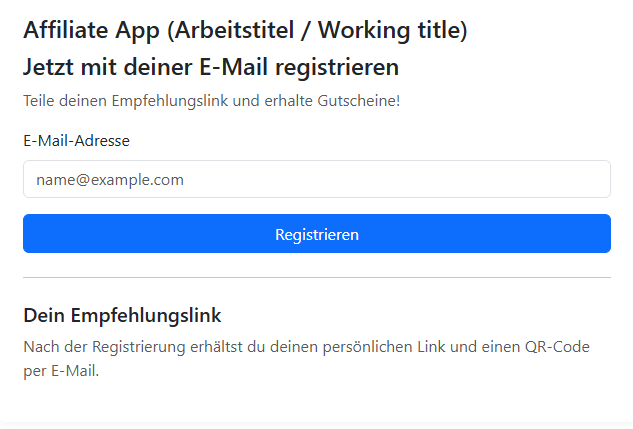
\includegraphics[width=0.8\linewidth]{Bilder/screenshots/form_blank.png}
    \caption{Leeres Formular}
    \label{fig:placeholder}
\end{figure}

\begin{figure}[H]
    \centering
    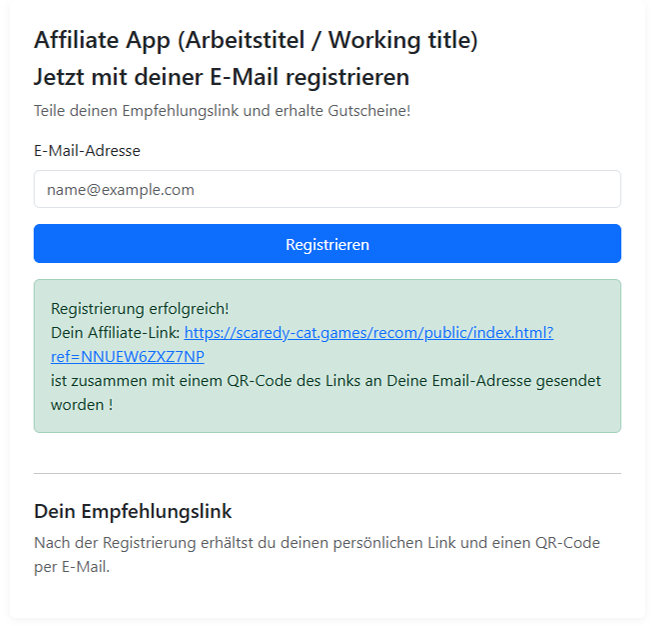
\includegraphics[width=0.8\linewidth]{Bilder/screenshots/form_registered.png}
    \caption{Erfolgreiche Registrierung}
    \label{fig:placeholder}
\end{figure}

\begin{figure}[H]
    \centering
    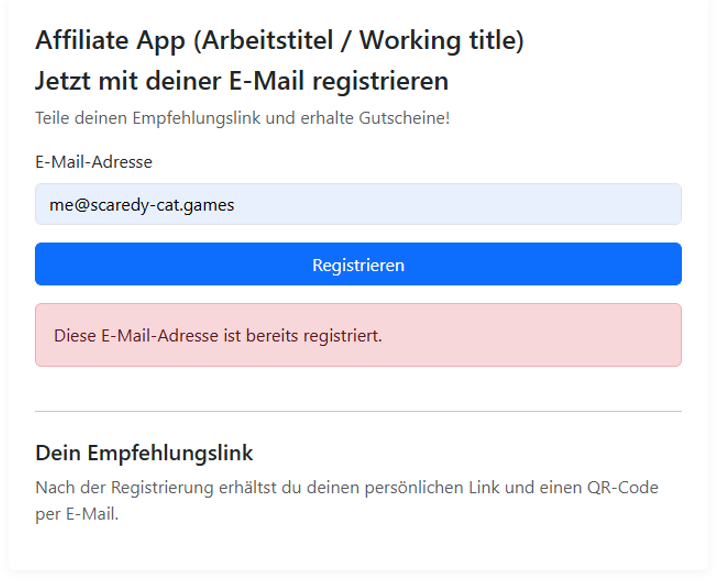
\includegraphics[width=0.8\linewidth]{Bilder/screenshots/form_already_registered.png}
    \caption{Fehlermeldung bei doppeltem Registrierungsversuch}
    \label{fig:placeholder}
\end{figure}

\subsubsection{Emails an Werber oder Geworbenen}
\begin{figure}[H]
    \centering
    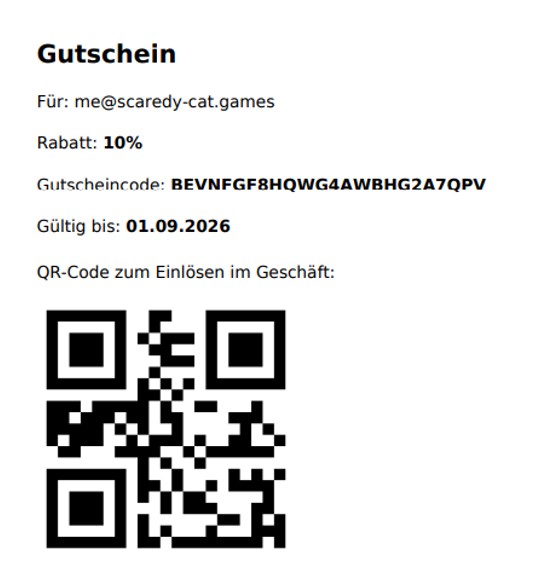
\includegraphics[width=0.5\linewidth]{Bilder/screenshots/email_voucher.png}
    \caption{Gutschein an Werber/Geworbenen}
    \label{fig:placeholder}
\end{figure}

\begin{figure}[H]
    \centering
    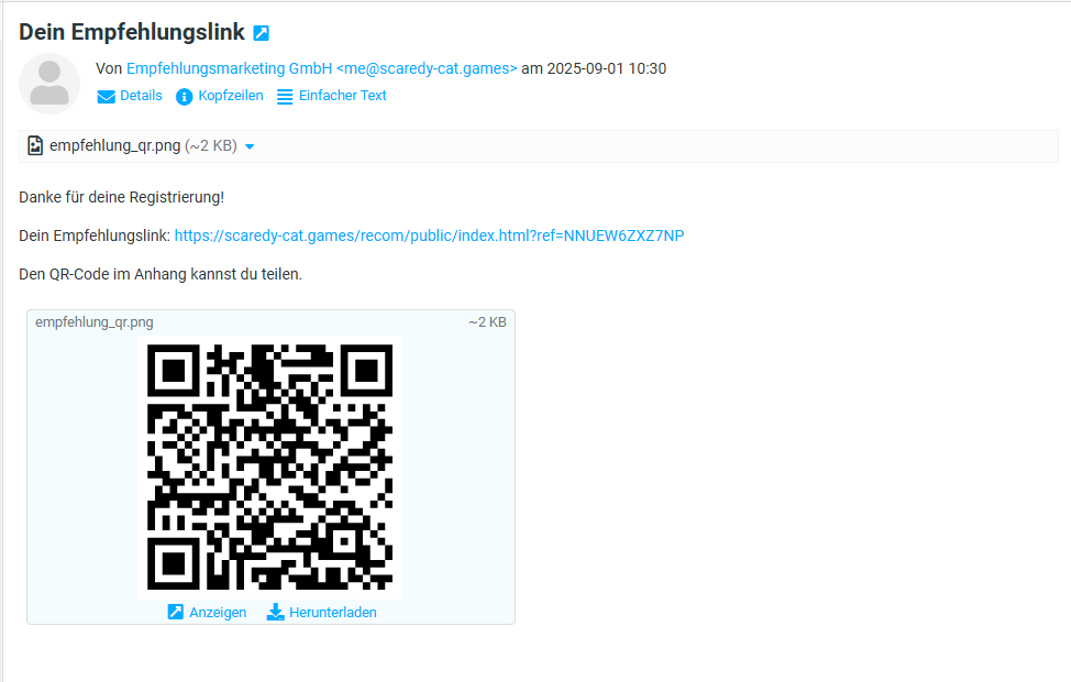
\includegraphics[width=1.0\linewidth]{Bilder/screenshots/mail_affiliate_link.png}
    \caption{Affiliate-Link und QR-Code an Werber/Geworbenen}
    \label{fig:placeholder}
\end{figure}


% \subsection{Oberflächenentwürfe}
\label{app:Entwuerfe}
\begin{figure}[htb]
\centering
\includegraphicsKeepAspectRatio{MockupModules.pdf}{0.7}
\caption{Liste der Module mit Filtermöglichkeiten}
\end{figure}

\begin{figure}[htb]
\centering
\includegraphicsKeepAspectRatio{MockupModul.pdf}{0.7}
\caption{Anzeige der Übersichtsseite einzelner Module}
\end{figure}

\begin{figure}[htb]
\centering
\includegraphicsKeepAspectRatio{MockupTag.pdf}{0.7}
\caption{Anzeige und Filterung der Module nach Tags}
\end{figure}

% \clearpage
% \subsection{Screenshots der Anwendung}
\label{Screenshots}
\begin{figure}[htb]
\centering
\includegraphicsKeepAspectRatio{tagliste.pdf}{1}
\caption{Anzeige und Filterung der Module nach Tags}
\end{figure}
\clearpage
\begin{figure}[htb]
\centering
\includegraphicsKeepAspectRatio{modulliste.pdf}{1}
\caption{Liste der Module mit Filtermöglichkeiten}
\end{figure}
\clearpage

% \subsection{Entwicklerdokumentation}
\label{app:Doc}
\begin{center}
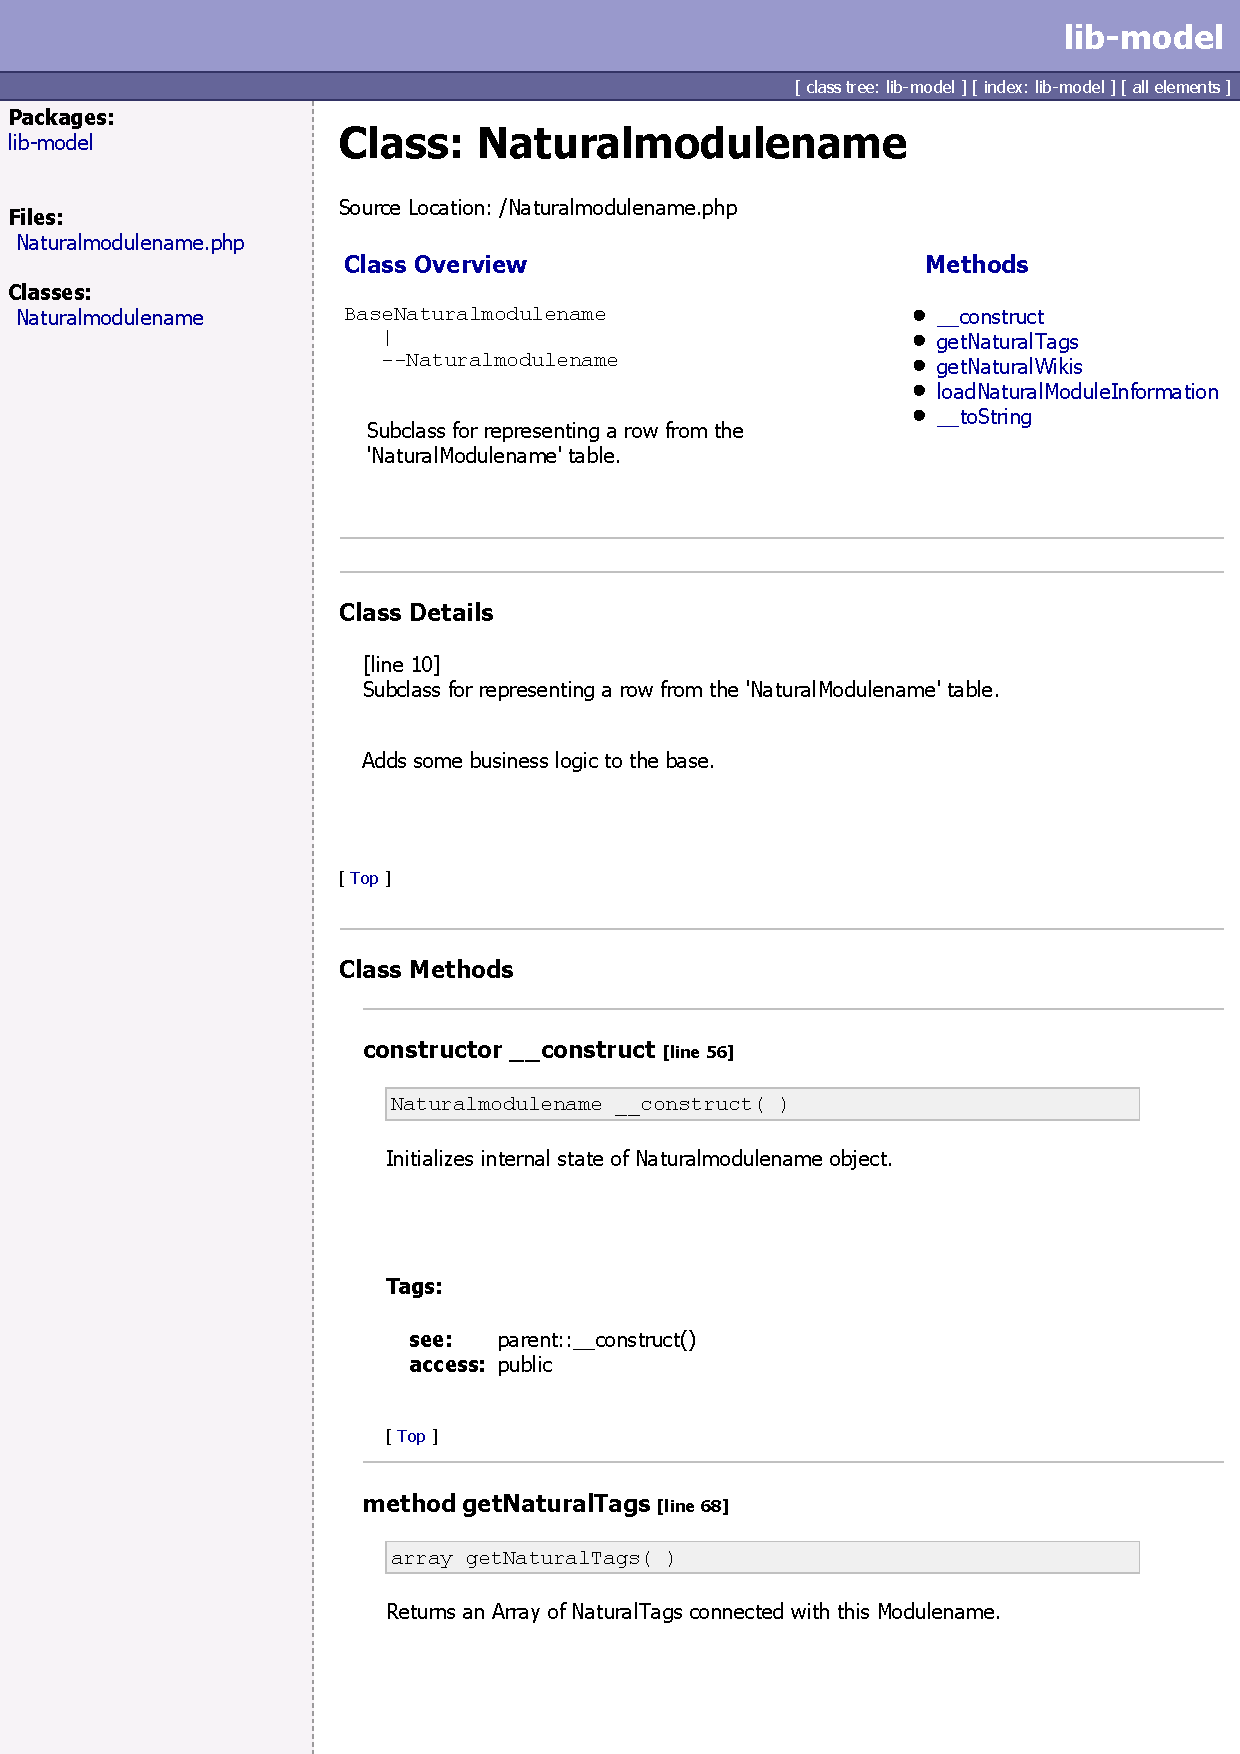
\includegraphics[page=1, width=0.9\textwidth]{doc.pdf}

\includegraphics[page=2, width=0.9\textwidth]{doc.pdf}
\end{center}

% \clearpage
% \subsection{Testfall und sein Aufruf auf der Konsole}
\label{app:Test}
\lstinputlisting[language=php, caption={Testfall in PHP}]{Listings/tests.php}
\clearpage
\begin{figure}[htb]
\centering
\includegraphicsKeepAspectRatio{testcase.jpg}{1}
\caption{Aufruf des Testfalls auf der Konsole}
\end{figure}


% \subsection{Klasse: ComparedNaturalModuleInformation}
% \label{app:CNMI}
% Kommentare und simple Getter/Setter werden nicht angezeigt.
% \lstinputlisting[language=php, caption={Klasse: ComparedNaturalModuleInformation}]{Listings/cnmi.php}
% \clearpage

% \subsection{Klassendiagramm}
% \label{app:Klassendiagramm}
% Klassendiagramme und weitere \acs{UML}-Diagramme kann man auch direkt mit \LaTeX{} zeichnen, siehe \zB \url{http://metauml.sourceforge.net/old/class-diagram.html}.
% \begin{figure}[htb]
% \centering
% \includegraphicsKeepAspectRatio{Klassendiagramm.pdf}{1}
% \caption{Klassendiagramm}
% \end{figure}
% \clearpage

% \subsection{Benutzerdokumentation}
\label{app:BenutzerDoku}
Ausschnitt aus der Benutzerdokumentation:

\begin{table}[htb]
\begin{tabularx}{\textwidth}{cXX}
\rowcolor{heading}\textbf{Symbol} & \textbf{Bedeutung global} & \textbf{Bedeutung einzeln} \\
\includegraphicstotab[]{weather-clear.png} & Alle Module weisen den gleichen Stand auf. & Das Modul ist auf dem gleichen Stand wie das Modul auf der vorherigen Umgebung. \\
\rowcolor{odd}\includegraphicstotab[]{weather-clear-night.png} & Es existieren keine Module (fachlich nicht möglich). & Weder auf der aktuellen noch auf der vorherigen Umgebung sind Module angelegt. Es kann also auch nichts übertragen werden. \\
\includegraphicstotab[]{weather-few-clouds-night.png} & Ein Modul muss durch das Übertragen von der vorherigen Umgebung erstellt werden. & Das Modul der vorherigen Umgebung kann übertragen werden, auf dieser Umgebung ist noch kein Modul vorhanden. \\
\rowcolor{odd}\includegraphicstotab[]{weather-few-clouds.png} & Auf einer vorherigen Umgebung gibt es ein Modul, welches übertragen werden kann, um das nächste zu aktualisieren. & Das Modul der vorherigen Umgebung kann übertragen werden um dieses zu aktualisieren. \\
\includegraphicstotab[]{weather-storm.png} & Ein Modul auf einer Umgebung wurde entgegen des Entwicklungsprozesses gespeichert. & Das aktuelle Modul ist neuer als das Modul auf der vorherigen Umgebung oder die vorherige Umgebung wurde übersprungen. \\
\end{tabularx}
\end{table}



\endgroup

\end{document}
